\documentclass{article}

% Language setting
% Replace `english' with e.g. `spanish' to change the document language
\usepackage[english]{babel}

% Set page size and margins
% Replace `letterpaper' with `a4paper' for UK/EU standard size
\usepackage[a4paper,top=2cm,bottom=2cm,left=3cm,right=3cm,marginparwidth=1.75cm]{geometry}

% Useful packages
\usepackage{amsmath}
\usepackage{graphicx}
\usepackage[colorlinks=true, allcolors=blue]{hyperref}
\usepackage{cleveref}

\usepackage[
  autocite    = superscript,
  backend     = bibtex,
  sortcites   = true,
%   style       = numeric,
  doi=false, url=true, isbn=false,
  maxcitenames=2, maxbibnames=2
  ]{biblatex}

\bibliography{references}

\renewcommand{\vec}[1]{\boldsymbol{#1}}
% \renewcommand{\hat}[1]{\hat{\vec {#1}}}

\graphicspath{{../imgs}}

\title{Effective dynamics of an aircraft}

\author{Art L. Gower and Matheus de Carvalho Loures}

\begin{document}
\maketitle

\begin{abstract}
    To plan optimal aircraft routes we can not completely solve and describe 3D fluid structure interaction. This would be computationally very intense and unnecessary. Instead, we need to capture the main features related to fuel consumption, ability to turn, and affects from the atmosphere such as drag and lift. To achieve this we develop effective dynamical equations, together with a simple numerical scheme to solve these equations. The method is simple enough to using nonlinear optimisation to plan routes with minimal fuel, or distance, or time.  
\end{abstract}

\section{Equations of motion}
The main forces acting on the aircraft are due to thrust, drag, lift, and a turning force. More accurately: an aircraft turns by rolling and then using lift, however we will not model these details, and instead have a turning force which is similar to a lift force.

\begin{figure}[ht]
    \centering
    \includegraphics[width = 0.4\linewidth]{"plane-sketch.png"}
    \caption{A sketch showing that the aircraft velocity vector is given by $\vec v$ (relative to the ground), and the velocity of the wind (relative to the ground) is given by $\vec u$. We approximate that the aircraft always points in the direction of travel.}
    \label{fig:plane-sketch}
\end{figure}

As it is impractical to solve for even the rigid body dynamics of the aircraft, which would allow for rotations, we assume that the aircraft always points in the direction of travel. See \cref{fig:plane-sketch} for a sketch. 

To describe the aircraft dynamics it is useful to use a local coordinate system with basis vectors:
\begin{align}
    & \vec e_v \quad \text{(the direction of travel)}
    \\
    & \vec e_r \quad \text{(radial direction from earth centre to aircraft)}
    \\
    & \vec e_p = \vec e_r \times \vec e_v  \quad \text{(perpendicular to travel direction)}
\end{align}
where we will only model the 2D dynamics and assume the altitude is fixed, so that $\vec e_v$ is always orthogonal to $\vec e_r$. Note that changes of altitude based on balance of lift with gravity can easily be accomodated without modelling the motion that leads to that change. 

There are two main forces on the aircraft, those that can be controlled by the pilot $\vec f$ and those that external $\vec w$. The forces that can be controlled are: 
\begin{equation}
    \vec{f} =  T(\dot{m}) \vec{e}_v + {L_p}(\vec v - \vec u, \alpha) \vec{e}_p  + {L_r}(\vec v - \vec u,\beta) \vec{e}_r,
\end{equation}
where $\dot m$ is the rate of change of mass in time (from using fuel), $v = |\vec v|$, $T(\dot{m},t)$ is the force from thrust, ${L_p}(v, \alpha)$ is a force which leads to turns in the $\vec e_p direction$, where $\alpha$ captures the amount the pilot tries to turn, and $L_r(v,\beta)$ are the lift forces, where $\beta$ is the amount to pilot tries to lift. 

A simple and effective choice for thrust is
\begin{equation}
    T(\dot{m}) = - \dot m C_{T} \quad \text{and} \quad 
    L_p (v, \alpha) = v^2 \alpha,
\end{equation}
where $C_T$ is a constant which describes how efficiently fuel burn $\dot m$ is converted into a thrust. More accurately, 
\[
C_T = \text{(exhaust velocity)} - \text{(relative airspeed)},
\] 
for subsonic flight \cite[Chapter 4]{anderson2005introduction}, where exhaust velocity is the speed of exhaust relative to the aircraft, and relative airspeed equals $|\vec v - \vec u|$ is the speed of air relative to the aircraft.

A simple and effective formula for the turning force is
\begin{equation}
    L_p (v, \alpha) = |(\vec v - \vec u) \cdot \vec e_v|^2 \alpha.
\end{equation}
In practive, turning is due to rolling and then lift. The forces that lead to rolling and lift are due to wind drag, which is proportional to the relative airspeed in the direction of travel. The variable $\alpha$ is bounded: $\alpha \in [-C_\alpha, C_\alpha]$, where the positive constant $C_\alpha$ depends on the type of aircraft.

The dynamics of the aircraft are now governed by balance of momentum:
% \begin{equation}
%     \vec{f}= \vec{w}(r,\vec{v},t) - T(\dot{m},t)\vec{e}_v+ \vec{L_c}(v(t), \alpha(t)) +\vec{L_u}(\vec{v}(t),\beta(t))
% \end{equation}
% We start supposing the the plane can only move in a spherical shell with coordinates $(\theta, \phi)$. We will write the problem in the coordinate of the perpendicular direction of the velocity ($\vec{e}_p$) and velocity direction ($\vec{e}_v$) in the spherical shell.
% The Thrust force in general coordinates is:
% \begin{equation}
%   - T(\dot{m},t) \vec{e}_v(t)
% \end{equation}
% observe that the normal to $\vec{e}_v(t)$ is $\vec{e}_p(t)=\vec{e}_r(t)\times  \vec{e}_v(t)$ in the sphere surface. The normal component normal to the sphere surface is $\hat{e}_r$. The force to turn on the surface is then
% \begin{equation}
%     \vec{L}_c(\alpha(t),t)=L_c(\alpha(t),v(t))\vec{e}_p(t)
% \end{equation}
% while the lift force to turn in the radial direction is 
% \begin{equation}
%     \vec{L}_u(\alpha(t),t)=L_u(\alpha(t),v(t))\vec{e}_r(t)
% \end{equation}
% So $\vec{f}$ is given by:
% \begin{equation}
%     \vec{f}= \vec{w}(r,t)   - T(\dot{m},v(t)) \vec{e}_v(t)+ L_c(\alpha(t),v(t))\vec{e}_p(t) + L_u(\alpha(t),v(t))(\vec{e}_r(t)))
% \end{equation}
% Now we write the movement equations on the there directions ($\vec{e}_v(t), \hat n(t),\vec{e}_r(t)$)
\begin{align}
    % \frac{dp}{dt}= \vec{f} \implies 
   \notag & \frac{d}{dt} (m(t) \vec{v}(t)) = \vec{f} + \vec{w} \implies
\\ \label{eqns:motion-vector}
    & \dot{m}\vec{v} + m \dot{\vec{v}} = T(\dot{m}) \vec{e}_v + {L_p}(\vec v - \vec u, \alpha) \vec{e}_p  + {L_r}(\vec v - \vec u,\beta) \vec{e}_r + \vec w,
% \implies
% \\
%     & \dot{m}(t)v(t)\vec{e}_v(t) +m(t)\dot v(t)\vec{e}_v(t) + m(t) v(t)\dot{\vec{e}_v}(t) = \vec{f}
\end{align}
where $\vec w$ are the forces due to external factors, such as the wind and altitude. It is generally a function of the relative airspeed $\vec v - \vec u$, however we do not need to give explicit forms for this forces, nor for the lift $L_r$ to simplify the equations of motion. 

To simplify \eqref{eqns:motion-vector} we need to write all expressions in terms of the local coordinate basis $\vec e_v, \vec e_p, \vec e_r$. First we assume that the external forces can be decomposed in the form:
\[
\vec w = w_v \vec e_v + w_p \vec e_p + w_r \vec e_r.
\]

Next we rewrite the expression:
\begin{equation} \label{eqn:mass-momentum}
    \dot{m}\vec{v} + m \dot{\vec{v}} = \dot{m}v \vec{e}_v + m \dot v \vec{e}_v + m v \dot{\vec{e}}_v.
\end{equation}
To rewrite $\dot{\vec{e}}_v$ we use the standard identities for basis vectors $\frac{d}{dt}(\vec{e}_v \cdot \vec{e}_v)=0$
% \begin{equation}
%   \frac{d}{dt}(\vec{e}_v \cdot \vec{e}_v)=0, \quad \frac{d}{dt} (\vec{e}_v \cdot \vec{e}_r)=0,  \quad \text{and} \quad \frac{d}{dt}(\vec{e}_v \cdot \vec{e}_p) = 0,
% \end{equation}
to conclude that $\dot{\vec{e}}_v$ is orthogonal to ${\vec{e}}_v$ and can be expanded in the form:
\[
\dot{\vec{e}}_v =  (\dot{\vec{e}}_v \cdot \vec{e}_p)\vec{e}_p + (\dot{\vec{e}}_v \cdot \vec{e}_r)\vec{e}_r,
\] 
which combined with \eqref{eqn:mass-momentum}, and the separation of the external forces, leads us to rewrite the equations of motion \eqref{eqns:motion-vector} in the form 
\[ 
a_v \vec e_v + a_p \vec e_p + a_r \vec e_r = 0.
\]
The above then implies that $a_v =0$, $a_p =0$, and $a_r =0$, which written in full become:
% \begin{equation}
%    \dot{\vec{e}_v}(t)=  -(\dot{\vec{e}_p}(t) \cdot \vec{e}_v)\vec{e}_p- (\dot{\vec{e}_r}(t) \cdot \vec{e}_v)\vec{e}_r
% \end{equation}
% \begin{equation}
%     \dot{m}(t)v(t)\vec{e}_v(t) +m(t)\dot v(t)\vec{e}_v(t) + m(t) v(t)( -(\dot{\vec{e}_p}(t) \cdot \vec{e}_v)\vec{e}_p- (\dot{\vec{e}_r}(t) \cdot \vec{e}_v)\vec{e}_r) = \vec{f}
% \end{equation}
% then we isolate the terms in each direction, getting three differential equations
\begin{align} \label{eqn:thrust-momentum}
    &  \dot{m} v + m \dot v = w_v + T(\dot{m}),
    \\
    \label{eqn:turn-momentum}
    &  m(t) v(t)({\vec{e}}_p \cdot \dot{\vec{e}}_v) = w_p + L_p(\vec{v}-\vec{u},\alpha),
    \\
    \label{eqn:lift-momentum}
    & m(t) v(t)({\vec{e}_r}(t) \cdot \dot{\vec{e}}_v)=w_r +L_r(\vec{v}-\vec{u},\beta).
\end{align}

\subsection{Forward marching numerical method}

Let us start by choosing a position $\vec x$ for the aircraft in a spherical coordinate system $(r,\theta,\phi)$ with
\[
\vec x = r [ \sin \phi \cos \theta, \sin \phi \sin \theta,   \cos \phi].
\]
Then the velocity vector of aircraft is given by $\dot{\vec x} = \vec v$, with $\vec v$ pointing in the direction of flight (relative to the ground). Rewriting in spherical coordinates we get
\[
\vec v = r \sin \phi  {\vec e_\theta} \dot \theta + r  {\vec e_\phi} \dot \phi, 
\]
by assuming that the altitude $r$ is fixed. Then, from the above we deduce that
\begin{equation} \label{eqn:update_thetaphi}
    r \sin \phi \dot \theta = \vec v \cdot {\vec e}_\theta  \quad \text{and} \quad 
r \dot \phi = \vec v \cdot {\vec e}_\phi.
\end{equation}
From the above we can see that it is convenient to write the components $\vec v$ in terms of the local coordinate system ${\vec e}_\theta, {\vec e}_\phi, {\vec e}_r$ coordinate system. That is, in the code, 
\[
\vec v[1] = \vec v \cdot {\vec e}_\theta, \quad 
\vec v[2] = \vec v \cdot {\vec e}_\phi, 
\quad 
\vec v[3] = \vec v \cdot {\vec e}_r.
\]
We can then use the equations \eqref{eqn:update_thetaphi}  to calculate $\theta(t+h)$ and $\phi(t+h)$ by substituting 
\[
\dot \theta = \frac{ \theta(t+h) - \theta(t)}{h} \quad \text{and} \quad 
\dot \phi = \frac{ \phi(t+h) - \phi(t)}{h},
\]
into \eqref{eqn:update_thetaphi} and solving for $\theta(t+h)$ and $\phi(t+h)$. For consistency, we have that the components of all vectors are given in terms of the local basis in the code.

The equations of motion (\ref{eqn:thrust-momentum} - \ref{eqn:lift-momentum}) can now be turned into a forward marching numerical method to predict the trajectory of the aircraft, which we briefly summarise below.

Equation \eqref{eqn:thrust-momentum} can be used to update the speed $v(t)$ by substituting
\[
\dot { v}(t) = \frac{{v}(t+h) - {v}(t)}{h},
\]
and then solving for ${v}(t+h)$. From the second equation \eqref{eqn:turn-momentum} we can update the direction $\vec {e}_v$ and as a consequence $\vec e_p$. To start
\[
\dot{\vec e}_v = a {\vec e}_p + b {\vec e}_r, 
\]
because $\dot {\vec e}_v$ is orthogonal to ${\vec e}_v$. Substituting the above into \eqref{eqn:turn-momentum} then leads to
\begin{equation}
 a =  {\vec{e}}_p \cdot \dot{\vec{e}}_v =  (w_p(r,v,t) + L_p(\alpha(t),v(t) ) / (m(t) v(t)).
\end{equation}
To obtain $b$ we use 
\begin{equation}
b = \dot{\vec e}_v \cdot  {\vec e}_r = - {\vec e}_v \cdot  \dot {\vec e}_r =  - {\vec e}_v \cdot  {\vec v} / r = - v / r,    
\end{equation}
where we also used the $\vec e_r = \vec r / r \implies \dot{\vec e}_r = \vec v / r$ for fixed $r$.



% \eqref{eqn:turn-momentum} we can update $\vec {e}_p$ and as a consequence $\vec e_v$. To start
% \[
% \dot{\vec e}_p = a {\vec e}_v + b {\vec e}_r, 
% \]
% because $\dot {\vec e}_p$ is orthogonal to ${\vec e}_p$. Equation \eqref{eqn:turn-momentum} gives us 
% \begin{equation}
%  a =  \dot{\vec{e}}_p \cdot \vec{e}_v = - (w_n(r,v,t) + L_c(\alpha(t),v(t) ) / (m(t) v(t)).
% \end{equation}
% To obtain $b$ we use 
% \begin{equation}
% b = \dot{\vec e}_p \cdot  {\vec e}_r = - {\vec e}_p \cdot  \dot {\vec e}_r =  - {\vec e}_p \cdot  {\vec v} / r = 0,    
% \end{equation}
% which is further explained below. 
% \[
% \vec{x}=r{\vec{e}}_r \Rightarrow \vec{v} =\dot{\vec{x}}=\dot{r}{\vec{e}}_r +r \dot{\vec{e}}_r \Rightarrow \dot{\vec{e}}_r=\frac{\vec{v}}{r} 
% \]
 
To summarise we can use the above to update the direction $\vec e_v$
\begin{equation}
    \vec e_v(t+h) = \vec e_v(t) + a h \vec e_p(t) - \frac{v h}{r} \vec e_r(t)
\end{equation}
where using the coordinate system $(\theta,\phi,r)$ we always have that $\vec e_r = [0,0,1]$. As we have made first order approximations in $h$ the norm of $\vec e_v(t+h)$ will only be approximately 1. It is better to correct this by taking $ \vec e_v(t+h)  \leftarrow  \vec e_v(t+h) / | \vec e_v(t+h) |$. Finally, we can then update the perpendicular direction:
\begin{equation}
    %    \quad \text{and} \quad 
    \vec e_p(t+h) = \vec e_r \times \vec e_v(t+h).
\end{equation}

%  and $\vec e_p$ through

% \textbf{Art: I suppose we have to normalise $\vec e_p(t+h) $ so that it's magnitude does not stray over time?}

\subsection{Optimal routes}

The simplest way to find optimal routes if through the shooting method. That is, a few initial guesses are made, and then a nonlinear optimiser will try different values for the control variables thrust $\dot m$ and aircraft turning $\alpha$ to achieve some goal. 

The most basic goal is to achieve a target destination $\vec x_B$. Let the start and end of the flight time be $t_A$ and $t_B$, so that the last position of a simulated flight is $\vec x(t_B$). Then we use a nonlinear optimiser to minimise:
\[
\min_{\vec \alpha, \dot{\vec m}} | \vec x(t_B) - \vec x_B|,
\]
where the control variables are
\[
\vec \alpha = [\alpha(t_A), \alpha(t_A+h), \ldots, \alpha(t_B)] \;\; \text{and} \;\; 
\dot{\vec m} = [\dot m(t_A), \dot m(t_A+h) \ldots, \dot m(t_B)].
\]

In practice, instead of controlling $\alpha(t)$ and $\dot m(t)$ for every time step, we can instead represent each of these as piece-wise constant functions, each with about 10 different steps, and then minimise for the total of 20 steps. This allows us to refine simulations by making $dt$ small while having a small number of control variables.

Naturally, we can also minimise the flight time as well as achieve the destination $\vec x_B$, which leads to the objective function:
\begin{equation} \label{eqn:objective-flight-time}
    \min_{\vec \alpha, \dot{\vec m}} c_t | t_B - t_A| + | \vec x(t_B) - \vec x_B|, \quad \text{(minimise flight time)}
\end{equation}
where $c_t$ is an appropriately chosen constant. To make the above robust, we should in fact non-dimensionalise each of the parts, and use a constant, such as $c_t$ to give the appropriate weighting. For example, \href{https://github.com/arturgower/AircraftRouteDynamics.jl/blob/354db5b80cef8d20cd8fcf031ec3f446823477eb/src/equations-motion.jl#L168}{in the code} the goal of minimising the total flight time 100 times less important than achieve the final destination.

We can choose to minimise any feature of the flight, such as minimising the total fuel used:
\begin{equation} \label{eqn:objective-fuel-use}
    \min_{\vec \alpha, \dot{\vec m}} c_t | t_B - t_A| - m(t_B). \quad \text{(minimise fuel use)}
\end{equation}
Below we will compare different flight routes which minimise flight time or fuel use.

\subsection{Code and Numerical examples}
Here we give a brief description of the code \cite{gower2025AircraftRouteDynamics} and examples. The code used to generate the examples in this report is from \href{https://github.com/arturgower/AircraftRouteDynamics.jl/tree/v0.0.1}{AircraftRouteDynamics v0.0.1}. Note the most recent version is here: \href{https://github.com/arturgower/AircraftRouteDynamics.jl/tree/main}{AircraftRouteDynamics.jl}, which may work differently then what is described below.

In the code AircraftRouteDynamics.jl a range of parameters of the aircraft and route can be given as shown in \Cref{fig:configure-aircraft}, as well as running a simulation. A more detail description of the parameters and setting up a simulation are given in the \href{https://github.com/arturgower/AircraftRouteDynamics.jl/blob/v0.0.1/README.md}{landing page}. Note the simulation result shown in \Cref{fig:one-route}, which uses a more elaborate wind pattern which imitates a tornado, took 280 microseconds on a regular PC.

\begin{figure}[h]
    \centering
    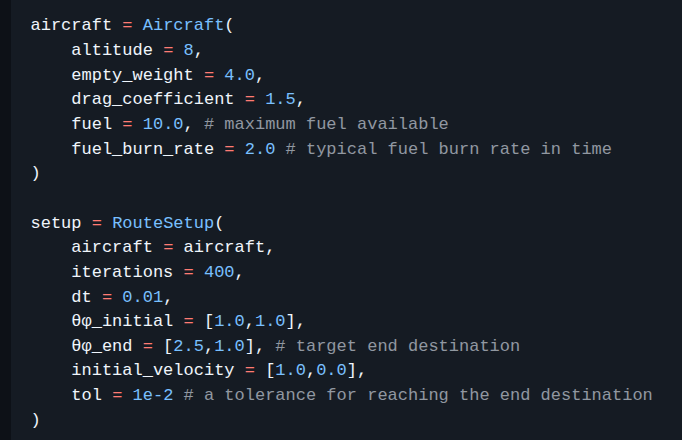
\includegraphics[width = 0.53\linewidth]{configure-aircraft.png}
    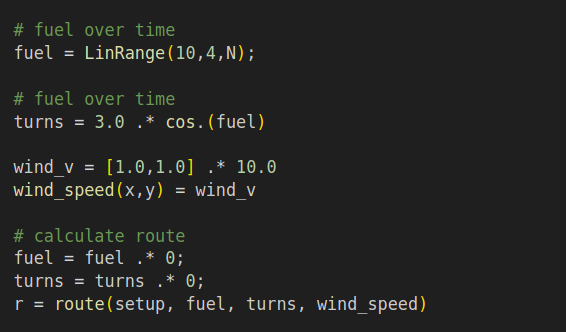
\includegraphics[width = 0.46\linewidth]{run-aircraft.png}
    \caption{An example of how to figure the package \href{https://github.com/arturgower/AircraftRouteDynamics.jl/tree/main}{AircraftRouteDynamics.jl} to run a simulation of one route. The parameters above are not realistic for a commercial aircraft.}
    \label{fig:configure-aircraft}
\end{figure}

\begin{figure}[h]
    \centering
    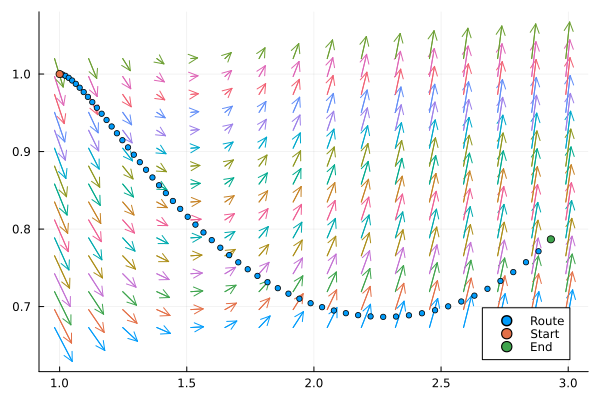
\includegraphics[width = 0.6\linewidth]{readme-1.png}
    \caption{Example of the simulation of one route, with the start and end point highlighted. Note that the end point does not match the one given in the parameters shown in \Cref{fig:configure-aircraft}. To achieve a specific end point you have to find an optimal route as specified below.}
    \label{fig:one-route}
\end{figure}

Finally, the package can find optimal routes through a shooting method. In essence, we give an initial guess for the fuel use (usually constant rate), turns (usually zero), and initial velocity. We then use a nonlinear optimiser to adjust these parameters to minimise either the flight time \eqref{eqn:objective-flight-time} or the fuel use \eqref{eqn:objective-fuel-use}.

\Cref{fig:compare-routes} compares routes that minimise flight time or fuel use for the case of a tornado like wind, whose strength is greatly exagerated to help visually distinguish between the two routes. All the configurations for these simulations are shown in the link: \href{https://github.com/arturgower/AircraftRouteDynamics.jl/tree/v0.0.1}{AircraftRouteDynamics v0.0.1} .

\begin{figure}
    \centering
    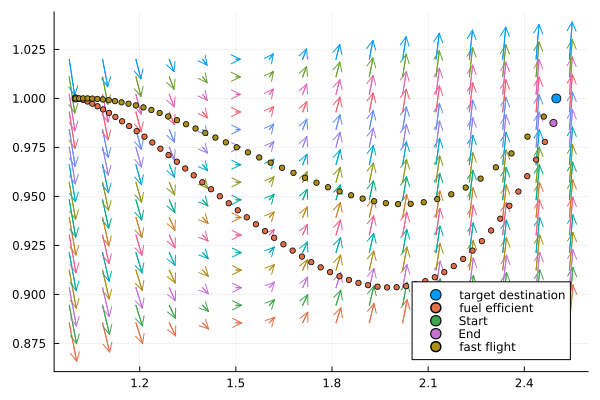
\includegraphics[width = 0.59\linewidth]{readme-5.png}
    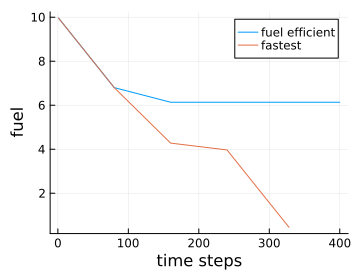
\includegraphics[width = 0.4\linewidth]{readme-6.png}
\caption{Compares two routes one which minimise fuel use and other which minimises total flight time. On the left we see that fastest flight time took a more direct route, while the fuel efficient route was longer but made better use of the wind. On the right we see how the fule efficient route used less fuel. Note wind strength was greatly exagerated.}
\label{fig:compare-routes}
\end{figure}


\section{Calculating the Lift coefficient to keep the aircraft at a certain Height}

\subsection{Lift coefficient above the tropopause}

The dynamics model above does not include changes due to changes in altitude. These changes would affect drag for example. However, it is simple to add changes of altitude into the model, without consider the full three-dimensional trajectory of the aircraft. Below we give some relevant formulas, but did not have enough time to integrate them in the model above or the code.  

The lift force is calculated as  \cite{nuic2004bada} 

\begin{equation}
    L_r= \frac{\beta }{2} \rho |(\vec{v}-\vec{u})\cdot \vec e_v|^2S
\end{equation}
Where $|\vec{v}-\vec{u}|$ is the speed of the plane related to the wind, $\rho$ is the air density, m is the mass of the plane, g is gravity , S is the area of the wing  projected at the plane normal to $\vec{e}_r$, and $\beta$ is the lift control parameter. From that we can see that the lift force is proportional to the air density. However the air density varies with the altitude of the aircraft. This dependece also can be approximatted by different formulas depending on the Altitude. For Heights above the tropopause  \cite{nuic2004bada} which is the altitude that separates the troposphere from the stratosphere ($\approx 11000$m) the density varies as

\begin{equation}
    \rho= \rho_{\text{trop}}e^{-\left( \frac{g}{RT_{\text{trop}}}(H-h_{\text{trop}}) \right)},
\end{equation}
where, $R$ is the gas constant  and the sub-index 'trop' means the tropopause value of the density,temperature, and altitude provided in \cite{nuic2004bada}. The pressure also follows the same behaviour.

\begin{equation}
    P= P_{\text{trop}}\mathrm{e}^{-\left( \frac{g}{RT_{\text{trop}}}(H-h_{\text{trop}}) \right)}.
\end{equation}
 

The force balance in $\vec{e}_r$ direction gives equilibrium of the plane at a constant altitude $H$. This allow us to determine the lift control variable $\beta$ if we wish to keep a constant altitude $H$. So the total external force on the direction $\vec{e}_r$ is 

\begin{equation}
    w_r=-mg -PA ,
\end{equation}
where $A$ is the projected area of the whole plane. Then the equation of motion in the $\vec{e}_r$ direction become
\begin{equation}
    -m\frac{v^2}{r}=-mg- PA +L_r
\end{equation}

\begin{equation}
     -m(t)\frac{v(t)^2}{r}=-mg-  P_{\text{trop}}\mathrm{e}^{-\left( \frac{g}{RT_{\text{trop}}}(H-h_{\text{trop}}) \right)}A +\frac{\beta }{2} \rho_{\text{trop}}\mathrm{e}^{-\left( \frac{g}{RT_{\text{trop}}}(H-h_{\text{trop}}) \right)} |(\vec{v}-\vec{u})\cdot \vec e_v|^2S
   \end{equation}
notice that $r=R_{\text{earth}}+H$ where $R_{\text{earth}}\approx 6378\text{km}$. Then the assumption that $R_{\text{earth}}>> H$ is reasonable to do, so we approximate $r\approx R_{\text{earth}}$ on the above 
\begin{equation}
    -m\frac{v^2}{R_{\text{earth}}}= -mg-  P_{\text{trop}}\mathrm{e}^{-\left( \frac{g}{RT_{\text{trop}}}(H-h_{\text{trop}}) \right)}A +\frac{\beta }{2} \rho_{\text{trop}}\mathrm{e}^{-\left( \frac{g}{RT_{\text{trop}}}(H-h_{\text{trop}}) \right)} |(\vec{v}-\vec{u})\cdot \vec e_v|^2S
\end{equation}
Isolating $H$  we have that
%\begin{equation}
%\Rightarrow     -m\frac{v^2}{R_{\text{earth}}} +mg= \left(-  P_{\text{trop}}A +\frac{\beta }{2} \rho_{\text{trop}} |\vec{v}-\vec{u}|^2S\right) \mathrm{e}^{-\left( \frac{g}{RT_{\text{trop}}}(H-h_{\text{trop}}) \right)}
%\end{equation}

%\begin{equation}
 % \Rightarrow \frac{-m\frac{v^2}{R_{\text{earth}}} +mg}{\left(-  P_{\text{trop}}A +\frac{\beta }{2} \rho_{\text{trop}} |\vec{v}-\vec{u}|^2S\right)}=  \mathrm{e}^{-\left( \frac{g}{RT_{\text{trop}}}(H-h_{\text{trop}}) \right)}    
%\end{equation}
%\begin{equation}
 % \Rightarrow \log \left(\frac{-m\frac{v^2}{R_{\text{earth}}} +mg}{\left(-  P_{\text{trop}}A +\frac{\beta }{2} \rho_{\text{trop}} |\vec{v}-\vec{u}|^2S\right)}\right)=  -\left( \frac{g}{RT_{\text{trop}}}(H-h_{\text{trop}}) \right)    
%\end{equation}

\begin{equation}
    H= - \frac{RT_{\text{trop}}}{g}\log \left(\frac{-m\frac{v^2}{R_{\text{earth}}} +mg}{\left(-  P_{\text{trop}}A +\frac{\beta }{2} \rho_{\text{trop}} |(\vec{v}-\vec{u})\cdot \vec e_v|^2S\right)}\right)+h_{\text{trop}},
\end{equation}
or isolating $\beta$ that
\begin{equation}
\beta=    \frac{2}{\rho_{\text{trop}}|(\vec{v}-\vec{u})\cdot \vec e_v|^2S} \left( \mathrm{e}^{\left( \frac{g}{RT_{\text{trop}}}(H-h_{\text{trop}}) \right)} \left( -\frac{m v^2}{R_{\text{earth}}}+mg\right) + P_{\text{trop}}A  \right)
\end{equation}
Depending on which parameter we wish to control. 

An important point to remember is that when the plane banks, a component of the lift contributes to the turn. However, this effect is not accounted for in our model due to a lack of available information.

\subsection{Lift coefficient below the tropopause}

Another formula can be used to approximate density and pressure below the tropopause as explained in the previous section. The air density at a certain altitude can be approximated as \cite{nuic2004bada}

\begin{equation}
    \rho= \rho_0 \left(\frac{T_0-\frac{6.5H}{1000}}{T_0}\right)^{-\frac{g}{k_TR}-1} \quad \text{and} \quad P=P_0\left(\frac{T_0-\frac{6.5H}{1000}}{T_0}\right)^{-\frac{g}{k_TR}},
\end{equation} 
where $P_0$, $\rho_0$ and $T_0$ are the values of pressure, temperature and densities of the atmosphere at the sea level. Also $k_T$ is the boltzman constant and R is the real gas constant.
So as in the previous section, the total external force on the direction $\vec{e}_r$ is 
\begin{equation}
    w_r=-mg -PA 
\end{equation}

where $A$ is again the projected area of the whole plane.

\begin{equation}
    -m(t)\frac{v(t)^2}{r}=-mg+ L_r -PA
\end{equation}

where again we can use the approximation
\begin{equation}
  \Rightarrow  -m\frac{v^2}{R_{\text{earth}}}= -mg- P_0\left(\frac{T_0-\frac{6.5H}{1000}}{T_0}\right)^{-\frac{g}{k_TR}}A +\frac{\beta }{2}\rho_0 \left(\frac{T_0-\frac{6.5H}{1000}}{T_0}\right)^{-\frac{g}{k_TR}-1} |(\vec{v}-\vec{u})\cdot \vec e_v|^2S
\end{equation}

\begin{equation}
\beta= \frac{2}{\rho_0 \left(\frac{T_0-\frac{6.5H}{1000}}{T_0}\right)^{-\frac{g}{k_TR}-1} |(\vec{v}-\vec{u})\cdot \vec e_v|^2S} \left(-m\frac{v^2}{R_{\text{earth}}} + mg+ P_0\left(\frac{T_0-\frac{6.5H}{1000}}{T_0}\right)^{-\frac{g}{k_TR}}A \right)
\end{equation}

With that we can obtain the value of the lift coefficient to keep the plane at a certain H below the tropopause.
\printbibliography

\end{document}